\documentclass[]{article}
\usepackage{float, graphics, graphicx}
\usepackage{listings}

\lstset{
	language=Java
}

\title{Lux: A Distributed Multi-GPU System for Fast Graph Processing}
\author{1665528-Emiliano Luci, 1665803-Federico Trombetti}

\begin{document}

\maketitle

\section{Introduction}
\subsection{Description of the problem}
Graph applications have a high ratio of random memory accesses to actual computation done and are often embarrassingly parallel. It thus makes sense to leverage an architecture with a very high memory bandwidth and a high number of computational units. Fortunately, GPUs clusters are a thing that exists. 

\begin{figure}[H]

	\centering
	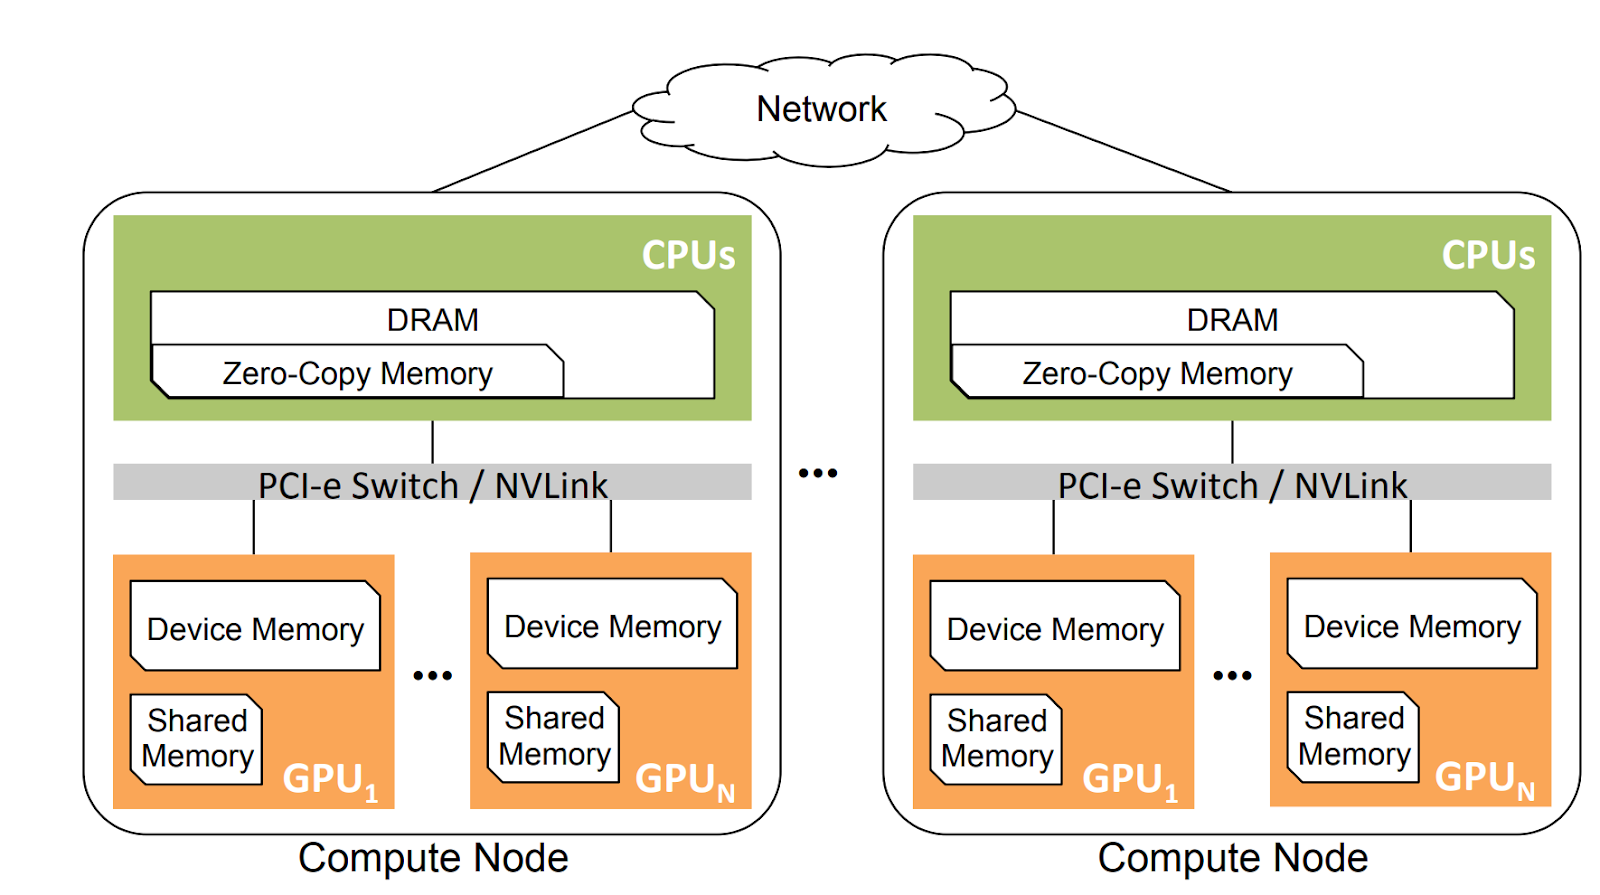
\includegraphics[width=0.7\linewidth]{gpu_cluster.png}
	\caption{The structure of a GPUs cluster}
	\label{fig:gpu_cluster}
\end{figure}
As we can see in Fig.\ref{fig:gpu_cluster} these systems have a very heterogeneous structure. In order to exploit their full potential one needs to build a framework that:
\begin{itemize}
	\item Distributes the graph efficiently amongst devices and within each device amongst the memories hierarchy.
	\item Find the best way to maximize locality in the memory access of the hierarchy.
	\item Minimize frequent uncoalesced updates to the graph ( i.e. minimize the need for inter-node and inter-device communication).
\end{itemize}

\subsection{Current approaches}
Many framework exists for graph processing. We will quickly go over them and where they present room for improvement:
\begin{itemize}
	\item \textbf{Distributed CPU-based systems}: CPUs are usually more limited in number of cores, large clusters imply greater message passing, access to DRAM is relatively slow and in any case not optimized for coalesced requests.
	\item \textbf{Single-Node CPU-based systems}: While this approach eliminates the need for inter-node communication it suffers from the same problems of untapped parallelization and memory bottleneck.
	\item \textbf{GPU-based systems}: the currently existing frameworks focus on single machine - multi GPUs systems and do not fully exploit the internal optimizations done by GPUs nor present a good approach to move data between memory hierarchies.
\end{itemize}
 
 \section{Contribution of the paper}
 We will now go through the framework structure and how the authors approached the problems presented.
 \subsection{Model of computation}
 
With some loss of generality, programs in Lux operate on immutable edges; vertices can be at most updated at each iteration. Furthermore all programs must implement the following interface:
 
\begin{lstlisting}[escapeinside={(*}{*)}]
interface Program (V, E) {
    void init ( Vertex v, Vertex v(*$_{old}$*) );
    void compute ( Vertex v, Vertex u(*$_{old}$*), Edge e );
    boolean update ( Vertex v, Vertex v(*$_{old}$*) );
}
\end{lstlisting}
The programs terminate when a convergence test succeeds.\\\\
Lux presents 2 iteration model for the execution of a program:
\begin{itemize}
	\item \textbf{Pull Model}: in this model the compute function operates on all the in-neighbours of each vertex, thus \textit{pulling} updates from them. The program terminates when vertices are no longer pulling any updates.
	\item \textbf{Push Model}: in this model the compute function operates on a subset of the out-neighbours of each vertex. Updates are \textit{pushed} from each vertex to its out-neighbours, issuing an explicit update. The program terminates when no vertex has any update to push.
\end{itemize}
The choice between the two models depends, of course, on the algorithm. If we're frequently updating large subset of the graph the pull model lets us exploit GPU optimizations such as aggregation of updates in shared memory. If, however, we're only updating a very small subset of the graph we don't want to pay the cost of operating on ALL of the vertices' neighbours at each iteration and, instead, we'd rather incur in the penalty of having to synchronize the small number of updates we explicitly push.

\subsection{Runtime}
\subsubsection{Memory utilization}
Consider the memory hierarchy presented in Fig.\ref{fig:gpu_cluster}. We know that:
\begin{itemize}
	\item The GPU shared memory is much faster than the Device memory which is faster than the Zero-copy memory
	\item The GPU shared memory is much smaller than the Device memory which is smaller than the Zero-copy memory
	\item Zero-copy memory is visible to ALL processors ( GPUs and CPUs).
\end{itemize}
Thus it makes sense that updates are first aggregated in the shared memory then pushed to the Zero-copy memory. While we gloss over the specifics of the task execution, this careful use of the different kind of memories constitutes the core strategy for reducing the time each GPU thread takes to complete, all other things being equal. Additionally Lux also leverages the CPUs to perform computation on data stored in Zero-copy memory when the graph won't fit in the Devices Memories.
\subsubsection{Graph Placement}
Since we have many units of computation we clearly need a partitioning of the graph. In this regard Lux employs a particularly appropriate strategy: instead of trying to do a very clever partitioning it uses a very fast edge partitioning approach. Vertices are assigned a unique number between $0$ and $|V-1|$. Partitions are assigned consecutive vertices such that each partition gets a fairly equal number of edges associated with the vertices. This partitioning is not only extremely fast to compute it also exploits an optimization done by GPUs for parallel consecutive memory accesses which are coalesced into a single range request which greatly reduces the time spent fetching data. Furthermore this partitioning offers two other benefits: we only need to keep a very small amount of information regarding each partition, namely the set of in/out-neighbours and their difference (which is the set of nodes that we need to update at each iteration); and, since Lux accepts graphs given in Compressed Sparse Row format it can ulteriorly speed up the computation of the splits needed to balance the partitions. This is great since it's almost guaranteed that graphs of billions of edges will be stored in a compressed format anyway.
\subsubsection{Load Balancing}
The partitioning adopted is indeed fair in the number of edges but it may not be balanced in the work that needs to be done on them. While an estimate of the load is computable a priori for some problems in most cases a dynamic approach is preferred. The approach Lux takes is based on the immediately available measures of the execution time at the end of each iteration. Lux can either perform global repartitions, i.e. amongst different nodes, or local repartition, i.e. amongst the devices in a single node. The criteria for repartitioning is loosely based on a measure of the variance of the execution time between computational units ( be it nodes or devices ). The gain obtained by a repartition is positively correlated with the variance. If the gain is greater than the cost of repartitioning, namely the cost of moving data around given a limited bandwidth then the operation is performed. The authors show that this approach reaches a good load balance in very few iterations on realistic ( power-law ) graphs.


\section{Critique}
We will now present some possible critiques to the paper.\\
The first one is on the restriction imposed on the program structure. This is similar to the criticism that has been expressed for MapReduce. Some problems will fit naturally in the interface provided but others must be awkwardly cast into it in order to make use of the framework.\\
Secondly Lux is essentially built to benefit from GPU clusters, and instead performs comparably to other frameworks for single node systems. This is not necessarily a critique (after all this is what it was designed for ) but it is to be considered if one doesn't have a GPU cluster just laying around. Although the authors show that such a system is still cost efficient the upfront expense is still considerably high.\\
Additionally let us consider Lux's execution model: at each iteration lots of updates, especially in the pull model, are passed around from device memory to Zero-copy memory. In fact, a big chunk of the time is indeed spent moving data around while the GPUs sit idle if they don't have Direct Memory Access. This poses another constraint when designing the algorithm as one must be extremely careful to minimize the duration of the compute phase. The memory bandwidth is also a hard cap to Lux's efficiency. That's not much of a problem if the graph snugly fits into the collective devices memory, however, having to store the graph in regular DRAM greatly diminishes Lux's speedup. This is not shown in the evaluation phase in the paper, where tests on single GPU systems have been done with graphs that indeed fit into a single device memory.\\
\end{document}
